\subsection{Opsætning webapplikation udvikling}
Dette afsnit har til formål at beskrive hvordan et udviklingsmiljø sættes op på en givet maskine så vider udvikling af systemet kan finde sted. Afsnittet forklare også hvilke tredjeparts teknologier der er anvendt og eventuelle afhængigheder.

For at kunne opsætte et udviklings miljø til client applikationen skal source koden først hente. Dette kan ske via git, skriv følgende kommando i terminalen.

\begin{lstlisting}[language=bash]
	$ git clone https://github.com/Opstrup/drone_frontend
\end{lstlisting}

\subsubsection*{Mappestruktur}
Dette underafsnit vil forklare om den overordnede mappe struktur i projektet og give en overordnet forståelse af angular client udvikling. \\

På figur \ref{fig:mappestruktur_client} ses mappestrukturen for client applikationen. Da Angular frameworket er opbygget over MVC\footnote{MVC model i forbindelse med Angular: https://docs.angularjs.org/guide/databinding} modellen er mappestrukturen opdelt så det afspejler denne model. I roden af projekt mappen findes to væsentlige file, app.js og index.html. app.js er settings filen for projektet, her bliver alle afhængigheder af projektet hentet ind og initialiseret, states i applikationen og dertilhørende controller bliver også registeret her\footnote{Information omkring app.js indstillingerne: https://docs.angularjs.org/guide/introduction}.\\
index.html er som kendt fra webudvikling den side som bliver hentet først ved et request, da Angular applikationer er et one paged app fungere det lidt specielt. Ved besøg af siden vil index side blive loaded samt javascript- og css-filer. Via Angular frameworket bliver alle andre sider så loaded ind i index siden, hvilket gøre applikationen meget hurtigt da filerne ikke skal indlæses igen.

\begin{figure}[H]
	\centering
	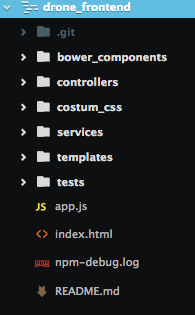
\includegraphics[width=0.2\textwidth]{Billeder/implementation/mappestruktur_client.png}
	\caption{Mappestruktur rod}
	\label{fig:mappestruktur_client}
\end{figure}

\textbf{bower\_components}\\
I denne mappe findes alle treide parts afhængigheder, i form af css og java script filer. Til håndtering af treide parts teknologier er der benyttet bower\footnote{http://bower.io/}, som er et package manager program til webudvikling.

\textbf{controllers}\\
I denne mappe findes alle controller\footnote{https://docs.angularjs.org/guide/controller} i systemet, som fungere på samme måde som kendt fra normal MVC.

\textbf{costum\_css}\\
Ud over bootstrap til håndtering af css'en, er der også blevet lavet nogle små filer med css kode. Disse filer findes i denne mappe.

\textbf{services}\\
I denne mappe findes alle services\footnote{https://docs.angularjs.org/guide/services} i systemet. Disse services indeholder alt buisness logikken i systemet og derved fungere som models i MVC modellen.

\textbf{templates}\\
I denne mappe findes alle html filerne for systemet, disser filer danner sammen med controllerne de views som bliver præsenteret i browseren\footnote{https://docs.angularjs.org/guide/templates}.

\subsubsection*{Udviklings miljø}
Opsætning af et udviklings miljø til client applikationen er rimelig simpel da source koden indeholder alt hvad der skal bruges for at kunne compile, der skal kun bruges en browser for at kunne starte applikationen. Til vider udvikling af applikationen vil det dog anbefales at der installeres nogle applikationer for at gøre udviklingen nemmere.

\textbf{Text editor}\\
Som alt andet web udvikling er det hele scripts som bliver kørt af browseren, derfor er der ingen specielle krav til et IDE af webudvikling. Nogle gode eksempler af text editor til web udvikling ville være Sublime eller Atom\footnote{Yderligere beskrevet i afsnittet om Server Opsætning}.

\textbf{Lokal web server}\\
For at applikationen fungere optimalt er det at anbefale at der installeres en web server på udviklerens maskine. Der er ikke nogle specielle krav til hvilke slags server. En simpel server kunne være en Apache server og for nem installation og opsætning kunne XAMPP\footnote{https://www.apachefriends.org/index.html} benyttes. Et andet eksempel på en web server kunne være en node.js server\footnote{http://nodejs.org/}. 

\textbf{Package management}\\
Som før nævnt er bower brugt til package management og det anbefales at der fortættes med dette da bower\footnote{http://bower.io/} selv downloader og installere de påkrævet filer, så udvikleren ikke skal tænke yderligere over dette.  

\newpage

\subsubsection*{Treide part teknologier}
Til udviklingen af web applikationen er der blevet brugt nogle treide parts teknologier, som er beskrevet yderligere i dette underafsnit.

\textbf{bootstrap}\\
Det populære bootstrap\footnote{http://getbootstrap.com/} css framework er benyttet til at give applikationen et flot design.

\textbf{ui-router}\\
Ui router\footnote{https://github.com/angular-ui/ui-router} er en applikation som er lavet til Angular frameworket som gør routing imellem div views meget simpel. 

\textbf{google-maps}\\
Google maps er blevet brugt til at vise kortet i applikationen og via google maps bliver der også hentet GPS-koordinater til de waypoints som dronen flyver efter. Google maps er ikke blevet benyttet som standart, men et angular applikation\footnote{https://angular-ui.github.io/angular-google-maps/} er blevet benyttet for at fungere bedre med den resterende kode.